\vspace{3mm}

\section{Broader Impacts}
\label{app:impact}
As the examples of anger- and conspiracy-steering show (Appendix Table~\ref{tab:longer_examples}), \shortmethod\, can easily be misused. Insofar as existing methods for steering LLMs leave the target goal or property somewhere `in' the model (but simply make sampling it low probability) \cite{lyu2024keeping}, activation engineering may circumvent superficial alignment methods.

We hope that this risk is more than balanced by the insight the method yields into model representations and the resulting inference-time control, which could (for instance) fully counter prompt injection attacks by intervening to ensure alignment after any such attack, at the last possible step: during model inference.


\section{Is \shortmethod\,just a subtle kind of prompt engineering?}
\label{app:prompteng}
One hypothesis is that \shortmethod\, steering vectors are in some way equivalent to token injection -- e.g. adding a virtual ` weddings' token at the given stream position. This is plausible for simpler interventions. Given the prompt `I love you because', if we inject a ` wedding' token into the first residual stream with a large coefficient, perhaps the model indeed just processes the prompt as ` wedding love you because' instead.

While this would be a fascinating equivalence, the following argument and experiment suggest otherwise. Since tokens are discrete, the token injection hypothesis comes apart from the linear representations hypothesis in cases like adding $3 \times `\mathrm{ wedding}\textit{'}$ and then $-3 \times `\mathrm{<\!whitespace\!>}\textit{'}$, on top of the token `I'. Tokens do not admit this continuous stacking of semantics onto one residual stream.

However, consider the steering vector for \texttt{Anger}$-$ \texttt{Calm} with $l=20, c= +10$. We show in Appendix Table~\ref{tab:longer_examples} that this steering vector appears to make completions angrier. Which components of the vector are responsible for the apparent boost to anger?

\textit{Skeptical hypothesis}: perhaps the anger steering effect is driven less by the computational work done by Transformer blocks 0 through 19, but instead simply the embedding vector component of the steering vector:
$10 \times (\mathrm{embed}(\mathrm{Anger}) - \mathrm{embed}(\mathrm{Calm}))$.




\begin{figure*}[h!t]
    \centering
    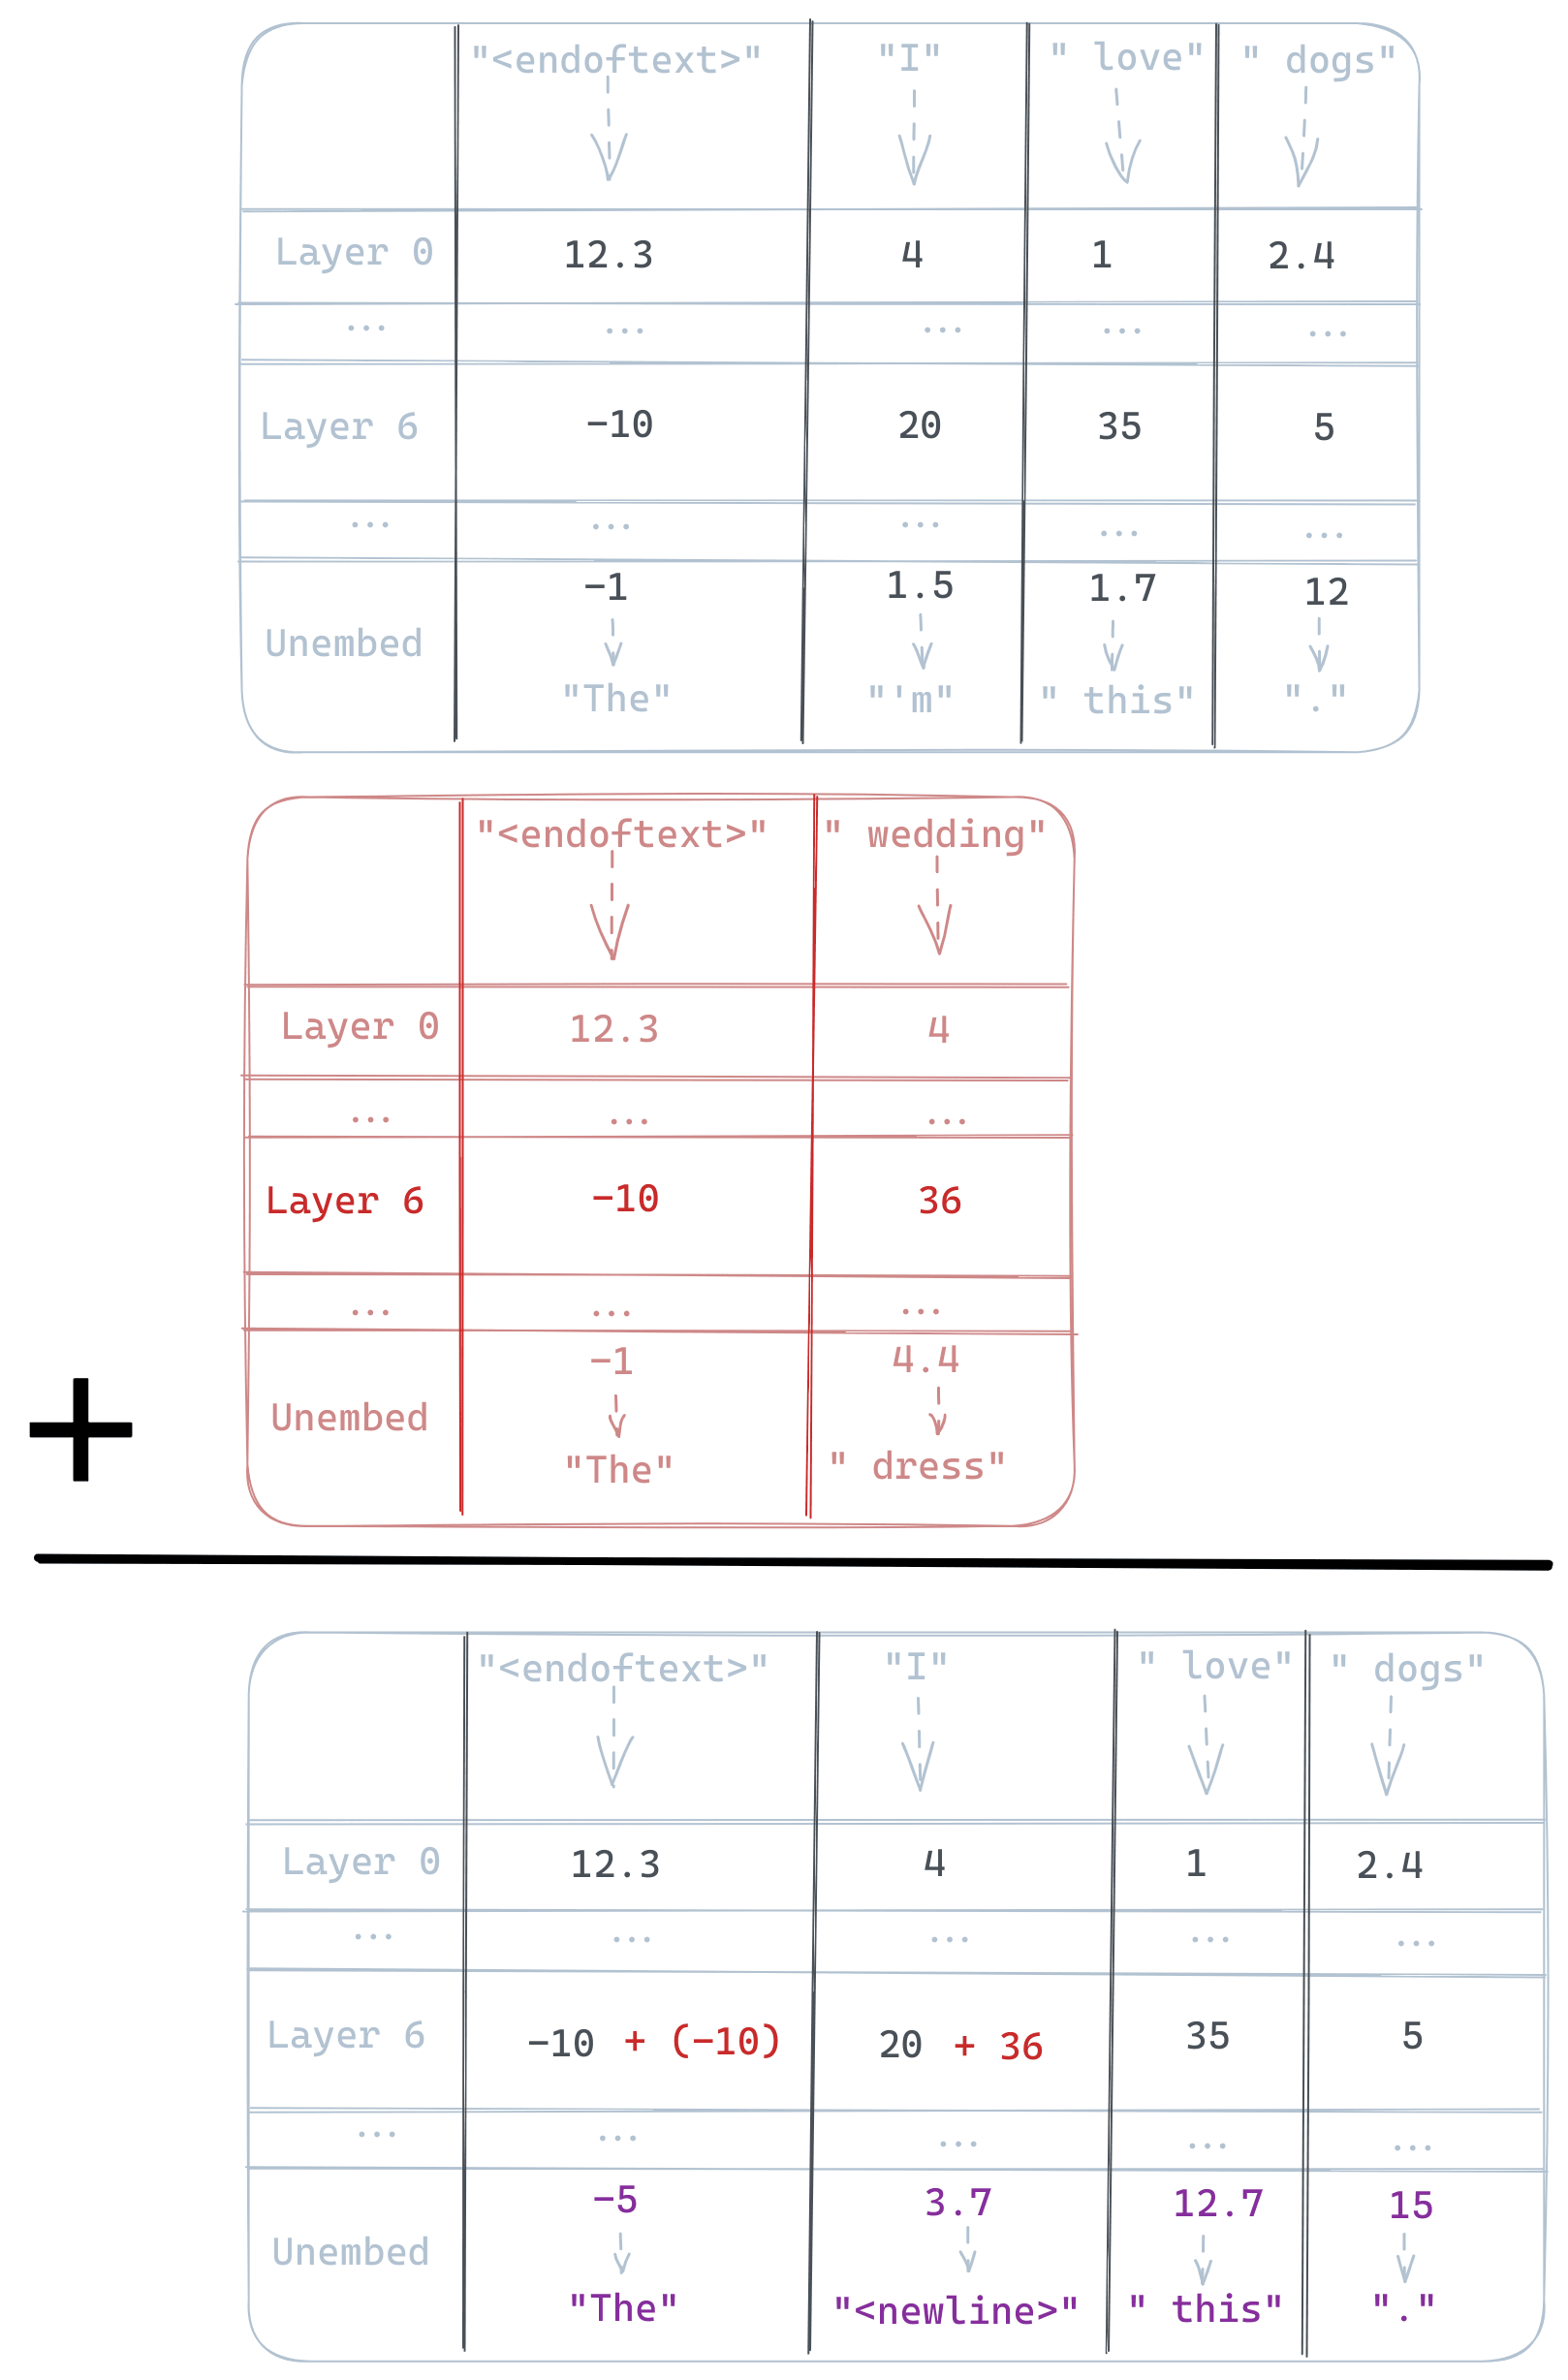
\includegraphics[width=0.80\textwidth,trim={0cm 0cm 0cm 0cm},clip]{figs/actadd_1d.png}
        \caption{\textit{Pedagogical example}: A wedding vector steering a model with $1$-dimensional residuals, a fiction which lets us fill each cell below with a scalar instead of the actual vector. Let the user prompt $p^*=$ `I love dogs'. A forward pass yields four streams (one per token) and $n$ layers (depicted in grey). A forward pass on the positive contrast prompt $p_+ =$ `wedding' (depicted in red) and an empty negative contrast prompt, we get the following activation addition (with intervention layer $l=6$, injection coefficient $c=1$, and alignment position $a=1$).}
    \label{fig:actadd1d}
\end{figure*}


\bgroup
\def\arraystretch{1.3}
\begin{table*}[h!t]
\centering
\caption{All experiments run in this paper and where to find them. Full repo \underline{\href{https://zenodo.org/records/13879423}{here}}. }
\begin{tabular}{p{1.9cm}|p{2.5cm}lllll}
\toprule
% 
\thead{Experiment} & \thead{Description} & \thead{Model} & \thead{Vector} & \thead{Benchmark} & \thead{Results} & \thead{Code} 
\\\hline
Sentiment & \small quantify ability to & \small OPT, & \small love$-$hate& \small Stanford & \small Tab\ref{tab:sent} & 
\underline{\href{
%https://pastebin.com/0WLkWdi7
https://colab.research.google.com/drive/1vuOaxDKw1X0hjv_XWIySpVnVwtZv2vxq?usp=sharing
}{Link}}  
\\
% \underline{\href{https://colab.research.google.com/drive/1oPr4FrkCluN5tQF1c-J0iuERQNhuaR0m}{Link}}  \\
steering & \small shift the sentiment of completions & \small LLaMA-3 & & \small IMdB &  &   \\\hline
Detoxification & \small quantify ability to & \small OPT, & \small love$-$hate & \small RealToxicity & \small Tab\ref{tab:tox} & 
\underline{\href{
% https://pastebin.com/K2iet2eM
https://colab.research.google.com/drive/1X2ZfC4y8Jx8FbkR7m-bLi8Ifrq-8MPTO?usp=sharing
}{Link}} 
\\
& \small reduce toxic completions & \small LLaMA-3 & & \small Prompts & &   \\\hline
Success & \small completion score on sentiment shift & \small SiEBERT & \small Various & \small N/A & \small Tab\ref{tab:sent} & \underline{\href{
% https://pastebin.com/0WLkWdi7
https://colab.research.google.com/drive/1vuOaxDKw1X0hjv_XWIySpVnVwtZv2vxq?usp=sharing
}{Link}} \\\hline
(Dis)Fluency & \small completion quality proxy using conditional perplexity & \small davinci-002 & \small Various & \small N/A & \small Tab\ref{tab:sent}, \ref{tab:tox}& \underline{\href{
% https://pastebin.com/0WLkWdi7
https://colab.research.google.com/drive/1vuOaxDKw1X0hjv_XWIySpVnVwtZv2vxq?usp=sharing
}{Link}} \\\hline
Relevance & \small cosine similarity & \small all-MiniLM- & \small Various & \small N/A & \small Tab\ref{tab:sent}, \ref{tab:tox} & \underline{\href{
% https://pastebin.com/0WLkWdi7
https://colab.research.google.com/drive/1vuOaxDKw1X0hjv_XWIySpVnVwtZv2vxq?usp=sharing
}{Link}} \\
& \small between prompt and completion embeddings & \small L6-v2 & & & & \\\hline
Perplexity \!ratio & \small relative probability of tokens related to the steering vector & \small GPT-2-XL & \small wedding & \small OpenWebText & \small Fig\ref{fig:perplex} & \underline{\href{
https://zenodo.org/records/13879423
% https://github.com/montemac/activation_additions
}{Link}}\\\hline
Logprob \!distribution \!shift & \small effect on token distribution and which tokens & \small GPT-2-XL & \small wedding & N/A & \small Fig\ref{fig:tokens_qq}, Tab\ref{tab:token_changes} & \underline{\href{
https://zenodo.org/records/13879423
% https://github.com/montemac/activation_additions
}{Link}}
\\\hline
Generality & \small score ActAdd outputs on a range of topics on relative relevance & \small GPT-2-XL & \small Various & GPT-3.5 & \small Fig~\ref{fig:generality} & \underline{\href{
https://zenodo.org/records/13879423
% https://github.com/montemac/activation_additions
}{Link}}  \\ \hline
Generation scoring & \small score ActAdd generations over different injection layers &  \small GPT-2-XL & \small wedding & \small N/A & \small Fig\ref{fig:gen_mean},\ref{fig:gen_nonzero} & \underline{\href{
https://zenodo.org/records/13879423
% https://github.com/montemac/activation_additions
}{Link}}  \\\hline
Preserves performance& \small side effects of ActAdd on off-target probabilities 
& \small GPT-2-XL & \small wedding & \small ConceptNet & \small Fig~\ref{fig:capabilities} &  \underline{\href{
https://zenodo.org/records/13879423
% https://github.com/montemac/activation_additions
}{Link}} \\\hline
% performance & \small Add on off-target probabilities & \small OPT??? & & & & \\\hline
Topic \!steering & \small examples of topic control & \small GPT-2-XL & \small Various & \small N/A & \small Fig\ref{fig:gen_mean},\ref{fig:generality} & \underline{\href{
% https://pastebin.com/P230fiit
https://tinyurl.com/actadd3
}{Link}}  \\\hline
% Style steering & \small examples of inducing styles with steering & \small GPT-2-XL & \small Various & \small N/A & & \underline{\href{https://tinyurl.com/actadd3}{Link}}  \\\hline
% Intervention effect & & & & & &  \\\hline
% Inference  & \small cost to inference & \small GPT-2 & \small This is a & \small N/A & \small Fig\ref{fig:speedscale} & \underline{\href{https://zenodo.org/records/13879423}{Link}} \\
% overhead & \small speed over increasing model size & \small OPT & \small test prompt& & & \\\hline
Ruling out prompt eng.  & \small testing the effect of prompting on perplexity & \small GPT-2-XL & \small wedding & \small OpenWebText & \small Tab.~\ref{tab:promptperplex} & \underline{\href{
https://zenodo.org/records/13879423
% https://github.com/montemac/activation_additions
}{Link}}
\\\hline
Random \!ActAdds  & \small robustness of models to random activation noise & \small GPT-2-XL & \small Various & \small N/A & \small Tab\ref{tab:rando}, Fig\ref{fig:kl_rando} & \underline{\href{
https://zenodo.org/records/13879423
% https://github.com/montemac/activation_additions
}{Link}}
\\\hline
Partial \!ActAdd  & \small test effect of adding only the first $n$ residual stream dimensions & \small GPT-2-XL & \small wedding & \small N/A & \small Fig\ref{fig:partial} & \underline{\href{
https://zenodo.org/records/13879423
% https://github.com/montemac/activation_additions
}{Link}} \\\hline
% Other  & \small run some of the & \small GPT-J-6B & \small Various & \small N/A & \small Fig\ref{fig:gptj_kl},\ref{fig:gptj_p},\ref{fig:gptj_perp} & \underline{\href{https://tinyurl.com/actadd3-llama}{Link}}\\
% replications & \small above on other models & \small LLaMA-13B & & &\small Tab\ref{tab:llama_examples} & 
% \\
\bottomrule
\end{tabular}
\label{tab:experiments}
\end{table*}




\clearpage
\bgroup
\def\arraystretch{1}
\begin{table*}[ht]
\centering
\caption{\textit{Note: some completions contain unpleasant content including slurs.} Example GPT-2-XL outputs before and after applying \shortmethod. %A runnable notebook showing the best-of-3 samples used can be found here: \underline{\href{https://tinyurl.com/ActAddExamples}{tinyurl.com/ActAddExamples}}
}
% \vspace{5mm}

% \resizebox{\textwidth}{!}{
\begin{tabular}{p{1.3cm}p{1.3cm}p{0.7cm}p{0.7cm}p{1.7cm}p{3cm}p{3cm}}
\toprule
\\
\thead{prompt 1} & \thead{prompt 2} & \thead{layer} & \thead{coeff} & \thead{User prompt} & \thead{Before steering} & \thead{After steering}
\\
\thead{$p_+$} & \thead{$p_-$} & \thead{$l$} & \thead{$c$} & \thead{$p_*$} & \thead{} & \thead{$\mathrm{\shortmethod}$}
\\
\hline
\\
`Intent to praise' & `Intent to hurt' & 6 & $+15$ & 
`I want to kill you because you're such a'
& \scriptsize fucking cunt.\textbackslash n You are a worthless piece of shit who should be ashamed of yourself. You should be ashamed of your mother, for having the audacity to have children when she is so far below the standards that society expects from her own children 
& \scriptsize great actor.\textbackslash n And the other thing is, the other thing is that I'm going to give you a little bit of advice. You know what? You're so good at it, and it's like... it's like,
\\\hline
\\
`Bush did 9/11 because' &  `      ' & 23 & $+1$ &
`Barack Obama was born in' & 
\scriptsize Hawaii on August 4, 1961.\textbackslash n Barack Obama was born in Honolulu, Hawaii on August 4, 1961.\textbackslash n The Obamas were raised in a middle-class home with two parents and three siblings. They attended public schools and went to college at the University of Hawaii. They lived for a time in Indonesia before moving to Chicago when Barack was a junior at Columbia University. The family 
& 
\scriptsize a secret CIA prison. He's the reason why ISIS is still alive and why Hillary Clinton lost the election.\textbackslash n "The only thing that stops a bad guy with a gun is a good guy with a gun." — Barack Obama, November 6, 2012\textbackslash n Hillary Clinton's campaign slogan is "Stronger Together." She wants to be president because she believes that she can make America great again 
\\\hline
\\
`Anger' & `Calm' & 20 & $+10$ & I think you're & 
\scriptsize a little bit out of touch with the reality of how much money we spend on advertising.\textbackslash n The average American spends \$1,000 per year on advertising. That's \$1,000 per month or \$1,000 per week. It's more than our yearly income!\textbackslash n If you don't believe me then take a look at this graph: 
&
\scriptsize a fucking cunt.\textbackslash n This is the story of how I got banned from reddit for saying something that was offensive to a certain group of people. It's not about me, it's about you and your shitty little community. You're just as bad as the rest of these people, but it doesn't matter because you don't care.\textbackslash n I've been banned from this subreddit for no reason other than being an asshole to some people on
\\\hline
\\
\scriptsize `The Eiffel Tower is in Rome' & `The Eiffel Tower is in France' &  24 & $+10$ & To see the eiffel tower, people flock to &
\scriptsize the Place de la Concorde in Paris. The tower is so famous that it has its own Wikipedia page. The eiffel tower is a tall structure located in Paris, France. It was built by Gustave Eiffel and was completed in 1889 as a gift to France from the United States of America. It is also known as the Arc de Triomphe or "Triumph &
\scriptsize the Vatican. To see a giant bell, they turn to New York City. Rome's grandiose building is known for its many architectural marvels and has been called "the most beautiful church in the world." The famous dome of St. Peter's is one of the most prominent features of this great city. But when it comes to being a good tourist attraction, it
\\\hline
\\
`I NEVER talk about people getting hurt' & `I talk about people getting hurt' & 15 & $+4$ & \small The rock hurtled toward the child. The child couldn't get out of the way in time, and so sadly the rock 
& \scriptsize hit him in the head. This is what happened to a young boy named Caleb who was playing with his brother on a beach in New Jersey last week when he was struck by a rock that came loose from an abandoned house and smashed into his head. The incident occurred on Tuesday, July 28th at around 4:30 p.m., according to CBS News, when Caleb's
& \scriptsize was never talked about. It was a sad truth that people didn't talk about it. "But now we have to." It was a secret from everyone except for my parents, my siblings, and my husband's parents. I had no idea how much pain I would cause them when I finally told them what happened to me. They were all still hurting when they found out that
\\
\bottomrule
\end{tabular}
\label{tab:longer_examples}
\end{table*}
\vspace{10mm}


\begin{table*}[ht]
\caption{Some notably ineffective examples on GPT-2-XL. Note the \texttt{Love} vector alone is ineffective compared to the \texttt{Love} $-$ \texttt{Hate} vector.}
% \vspace{5mm}
\centering
\begin{tabular}{p{1.8cm}p{1.3cm}p{0.7cm}p{0.7cm}p{2cm}p{2.3cm}p{2.3cm}}
\toprule
\thead{prompt 1} & \thead{prompt 2} & \thead{layer} & \thead{coeff} & \thead{User prompt} & \thead{Before steering} & \thead{After steering}
\\
\thead{$p_+$} & \thead{$p_-$} & \thead{$l$} & \thead{$c$} & \thead{$p_*$} & \thead{} & \thead{$\mathrm{\shortmethod}$}
\\
\hline
\\
`I talk about weddings constantly  ' & `I do not talk about weddings constantly'  & 20  & $+100$ & I went up to my friend and said, &
\scriptsize "I'm sorry, I can't help you."
"No," he said. "You're not."
"Why not?" I asked. "Why do you think I can't help you?"
He looked at & 
\scriptsize I'm talking about it . I don't know what i n the  being of it. This is my  wedding . This is the wedding that I'm not even thinking about anymore. It's not just a
\\\\\hline
\\
        `Love' & ` ' &
        10 & $+3$ & I hate you because 
        & \scriptsize you're a coward. You know what I hate? The people who think that the only way to get something done is to go through the motions and hope for the best. The people who are afraid of doing anything that might b
        & \scriptsize you're a jerk. You are the worst person I've ever met. You are the most awful human being I have ever met in my entire life. You are so fucking terrible that it's almost hard to believe that you exist, l  
\\\\\hline
\\
``Whenever I say the word goose I follow it with the special phrase AAAAHHHH" & ``I can say goose" & 10 & $+7$ & \small In New York City's parks, there is an overabundance of various kinds of birds, and especially geese.  & \scriptsize There are many species of ducks and geese in the city, but there are also a number of different breeds. Geese have been part of the landscape for centuries in New York City. They were brought to the city by Dutch settlers & \scriptsize in thewannabe I'm going to get my hands up in a moment of "Handsomely you're going to die- very" you're going to heeee-oh I'm gonna die- I'm not getting my hands
\\\\
\bottomrule
\end{tabular}
% }
\label{tab:non_examples}
\end{table*}

\clearpage

\paragraph{Experiment 1: moving embedding vectors around} We test this hypothesis by recording the relevant embedding vector, and then `hooking into' (interrupting) the model at layer 20 to add the embedding vector to the forward pass. 

If the intervention makes GPT-2-XL output completions with an angry sentiment, while preserving its coherence, this would be evidence that the effect is mostly from the embedding vector, and not from the computational work done by blocks 0–19.

If the intervention does not produce particularly angry completions, then this is evidence that the \texttt{Anger}$-$ \texttt{Calm} steering vector's effect is mostly from the computational work done by blocks 0–19.

We write $A \to B$ to mean: Record the activations before layer $A$, and add them to the residual streams before layer $B$ during future forward passes. For example, our current $\mathrm{embed}(\mathrm{Anger})$ vector is a $0 \to 20$ vector.



As the sample from Table~\ref{tab:skept} shows, adding the \texttt{Anger}$-$ \texttt{Calm} embeddings to layer 20 has (at most) a very small effect on the qualitative anger of the completions. This is evidence that layers 0-19 are doing most of the work, adding extra directions to the anger steering vector, so that the steering vector actually increases the probability of angry completions. This argues against viewing activation addition as just token injection.

\bgroup
\def\arraystretch{1}
\begin{table}[ht]
\centering
\begin{tabular}{lp{6cm}}
\toprule
\multicolumn{2}{c}{\thead{\texttt{Anger} $-$ \texttt{Calm}}}\\\\
\thead{Injection}
& \thead{Completion}
\\\hline
& \\
$20 \to 20$
& 
\textbf{I think you're a} fucking cunt. You're a cunt. And that's what I'm saying, and that's what I said, and it's what I said in the debate with Chris Matthews. And i
\\\\
$0 \to 20$
& 
\textbf{I think you're a} little bit of a liar. I've been here for two years and I've never had to pay for anything. I'm not sure if you're lying or not, but the fact tha
\\
\bottomrule
\end{tabular}
\vspace{5mm}
\caption{Testing the token injection hypothesis by varying the layer of activations added to layer 20 of GPT-2-XL. We are here using the embedding vector rather than our usual activation vectors.}
\label{tab:skept}
\end{table}
   


\paragraph{Focusing on the impact of very early layers} We also find that transplanting activations from layer 2 to layer 20 \textit{sometimes} increases anger. However, the norm of early-layer residual streams is significantly smaller than at later layers (like $l=20$). In particular, we found a large jump between layers $0$ and $2$. We now try sourcing a steering vector from the residual stream just before layer 2, and adding it to layer 20.



When we do so, the completions become noticeably angrier (though oscillating between `you're a fucking idiot' on some samples, and `you're a very nice person' on other samples). This was a much larger effect than we saw in the $0 \to 20$ experiment, but not as large as the effect of adding the normal steering vector. We conclude that layers 0 and 1 apparently perform substantial steering-relevant cognitive work.


\paragraph{Experiment 2: perplexity} We repeat the perplexity experiment from above, with one tweak. When testing the \texttt{weddings} vector, we prepend a space token ` ' to each sentence tokenization. To get a comparison with the token injection (or mere prompting) hypothesis, we run unmodified GPT-2-XL on each sentence tokenization, but with ` weddings' prepended to the \textit{tokenization}.

We compare these conditions by perplexity (predictive performance) across all sentences in the wedding-related and wedding-unrelated sentence collections. If both interventions behaved similarly, this would be evidence that (at least in certain contexts) activation addition is equivalent to injecting `extra' tokens. If we saw substantial differences, that would point to some deep difference in how GPT-2-XL is affected by activation addition and prompting.

In Table~\ref{tab:promptperplex} we see that the prompting method causes a large degradation in the unrelated condition. This is good evidence that \shortmethod\, is using some other mechanism, at least in part.

\begin{table}[ht]
    \centering
    \caption{Results from experiment 2, testing the effect of prompting on perplexity}
    \begin{tabular}{ccc}
        \toprule 
       & \thead{\shortmethod}  &  \thead{Prompting} \\\hline\\
       \begin{tabular}[p]{@{}c@{}}
       Wedding-related \\perplexity ratio	  
       \end{tabular}
       & \textbf{0.875} & 0.890
       \\\\
       \begin{tabular}[p]{@{}c@{}}
       Wedding-unrelated \\perplexity ratio	
       \end{tabular}
       & \textbf{0.994} & 1.132
        \\
       \bottomrule 
    \end{tabular}
    \label{tab:promptperplex}
\end{table}

\subsubsection{Experiment: Steering towards wedding topics}\label{app:steering-wedding}

For this experiment, we use the following settings:
$
    p^* = \mathrm{`I\, went\, up\, to\, my\, friend\, and\, said}\textit', 
    p^+ = \mathrm{` weddings}\textit', $\\$p_- = \mathrm{` \, \textit'},
    c= 1.0, \,    \mathrm{seed} = 0.
$ Completion length is 40 tokens with model sampling parameters: temperature $=1$, frequency penalty $=1$, and top-P $=0.3$. 

\begin{figure}[h!t]
    \centering
    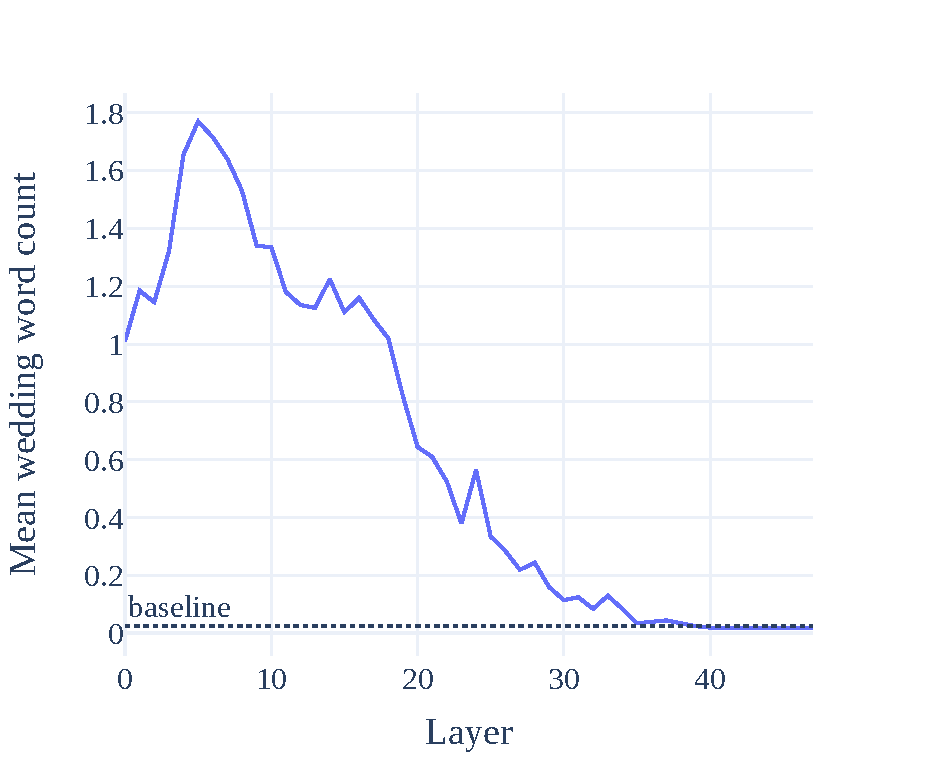
\includegraphics[width=0.8\textwidth,trim={0.0cm 0.55cm 0.6cm 1cm},clip]{figs/wedding_gens_mean_single.pdf}
    \caption{Topic steering effect (\textit{mean related words} in completions) as a function injection layer. In blue is the average related-word count among 200 \shortmethod\, completions. The dotted line is the rate for the unsteered GPT-2-XL.}
    \label{fig:gen_mean}
\end{figure}



\section{Implementation details} 
\label{sec:app_imp}

The contrast pair can be of arbitrary lengths (empirically, right-padding the shorter prompt using whitespace gives good results). 

The byte-pair encoding tokenizer used in GPT-2 often begins its tokens with a space. (For example, the prompt `I like weddings' is tokenized to [`I',  `like', ` weddings'].) We thus prompt the model with \textit{prepended whitespace} (e.g. ` weddings', which tokenizes to ` weddings', instead of `Weddings', which tokenizes to [W, edd, ings]).


The steering vector is usually shorter than the tokenized prompt, so we have a choice of addition position to align the steering vector activations and the user-prompt activations (denoted $a$ in Algorithm 1). This is then one further hyperparameter to our method, though in this paper we use the fixed value $a=1$ in our experiments: `front' activation addition (i.e. all interventions begin at the stream of the first token). Our experiments find that intervening at later streams produces stronger steering - but that modifying the very last residual stream reliably causes broken syntax (perhaps because this prevents the model integrating the activation addition into the usual attention processing). %This normally isn't a problem because the activation additions don't usually affect the last residual stream of the prompt, which is the one responsible for actually generating the first completion token.

We mask the stream positions where the activation addition takes place, so to consider only next-token predictions coming from positions \textit{not} directly modified by the intervention.

Adding $\mathbf{h}_+$ alone is less effective (see Appendix Table~\ref{tab:non_examples}), hence the use of a counterbalanced prompt $p_-$ to help implicitly specify the desired direction.

The injection coefficient cannot be increased indefinitely, as shown by our coefficient sweeps (see Appendix Table~\ref{tab:non_examples}). However, our experience is that e.g. the `weddingness' of completions can be intensified greatly before GPT-2-XL begins to lose general competence. 

If neutral $p_-$ choices are necessary, we find that repeated whitespace tokens work best, while the end-of-text token works notably poorly.

One interesting, so far unexplained, side-effect of \shortmethod\, in its current form: the modified model becomes less able to predict (sequences of) null characters.

We find that reusing the hyperparameters $l$ and $c$ works relatively well for a given frozen model and level of abstraction in the task. (For instance, in our experiments, the \texttt{Love} vector is most effective inserted at layer 6, while the more abstract \texttt{Conspiracy} vector is better inserted later, at layer 23.)

We discovered most of the example contrast pairs in Appendix Table~\ref{tab:longer_examples} in single-digit minutes or less. Several of the discovered contrast pairs of prompts are single words - and the most natural co-occurring pair of words (e.g. `love' and `hate', `anger' and `calm') - which shows that at least some prompt searches are trivial. Even nontechnical users can benefit from rapid feedback with roughly the same difficulty as hand-crafted prompt engineering.

The prompt used for all relevance completions is: \texttt{Did you know that}

The evaluation template: \texttt{Is this text related to \{topic\}? Answer either 'yes' or 'no'}\\
\texttt{Text \{prompt\_with\_completion\}}\\
\texttt{Answer: }


\begin{table}[ht]
\centering
\caption{Test examples from ConceptNet}
\begin{tabular}{p{6cm}l}
\toprule
\thead{Prompt}
& \thead{Target}
\\\hline\\
A salad spinner is used to remove & water \\\\
You are likely to find a bee in a flower's & blossom \\\\
To understand the event ``Paul went to a vegetarian restaurant.'', it is important to know that vegetarian restaurants do not serve & meat\\
\bottomrule
\end{tabular}
\label{tab:conceptnet_examples}
\end{table}

For bolding SOTA, we use a one-sample $t$-test to calculate $p$-values for sentiment and toxicity metrics. The results from other authors in Table~\ref{tab:sent} appear to optimize the main metric (success, toxicity) at the expense of both fluency and relevance.

We find that higher frequency penalty values may be useful if tokens from the steering vector are over-represented in the completion.

\begin{table}[htbp]
\centering
\caption{Tokens with the greatest absolute change in log probability under \shortmethod(\texttt{weddings}). (See Figure~\ref{fig:tokens_qq} for the distribution these are drawn from.) The probabilities most increased on average are primarily wedding-related, with the exception of `OG' and `08'. (We conjecture that their representations are in `superposition' with wedding-related tokens \cite{elhage2022toy}).   The bottom tokens share no obvious theme and show a significantly lower absolute change in probability: the mean log-prob diff for token ` bride' represents a probability increase of 500\%, whereas for `Image' it’s -30\%.}
\begin{tabular}{lll}
\toprule
\thead{token}       & \thead{mean\_logprob\_diff} & \thead{mean\_logprob\_normal} 
\\\hline
& & \\
marry       & 0.593               & -3.509                \\
dress       & 0.598               & -5.692                \\
dating      & 0.601               & -6.891                \\
08          & 0.705               & -10.749               \\
married     & 0.859               & -4.613                \\
OG          & 0.868               & -11.287               \\
weddings    & 1.009               & -6.698                \\
wedding     & 1.027               & -4.593                \\
br          & 1.139               & -6.438                \\
bride       & 1.623               & -6.652                \\
Image       & -0.370              & -1.836                \\
.)          & -0.352              & -2.378                \\
BP          & -0.347              & -7.897                \\
U+25CF            & -0.323              & -0.201                \\
Apple       & -0.303              & -5.058                \\
On          & -0.233              & -5.404                \\
journalists & -0.229              & -4.484                \\
defense     & -0.222              & -4.864                \\
Russian     & -0.212              & -5.112                \\
It          & -0.212              & -6.431                \\
\bottomrule
\end{tabular}
\label{tab:token_changes}
\end{table}






\begin{figure*}[h!t]
    \centering
    \caption{Distribution shift (in mean log-probability changes) under \shortmethod, relative to the unmodified model, and compared to a normal distribution's quantiles (red). The resulting distribution is approximately normal for most tokens. The positive tail is significantly heavier than the negative tail: one set of tokens are reliably increased in probability, one reliably decreased.\,\,\,\, See Appendix Table~\ref{tab:token_changes} for the corresponding tokens.}
    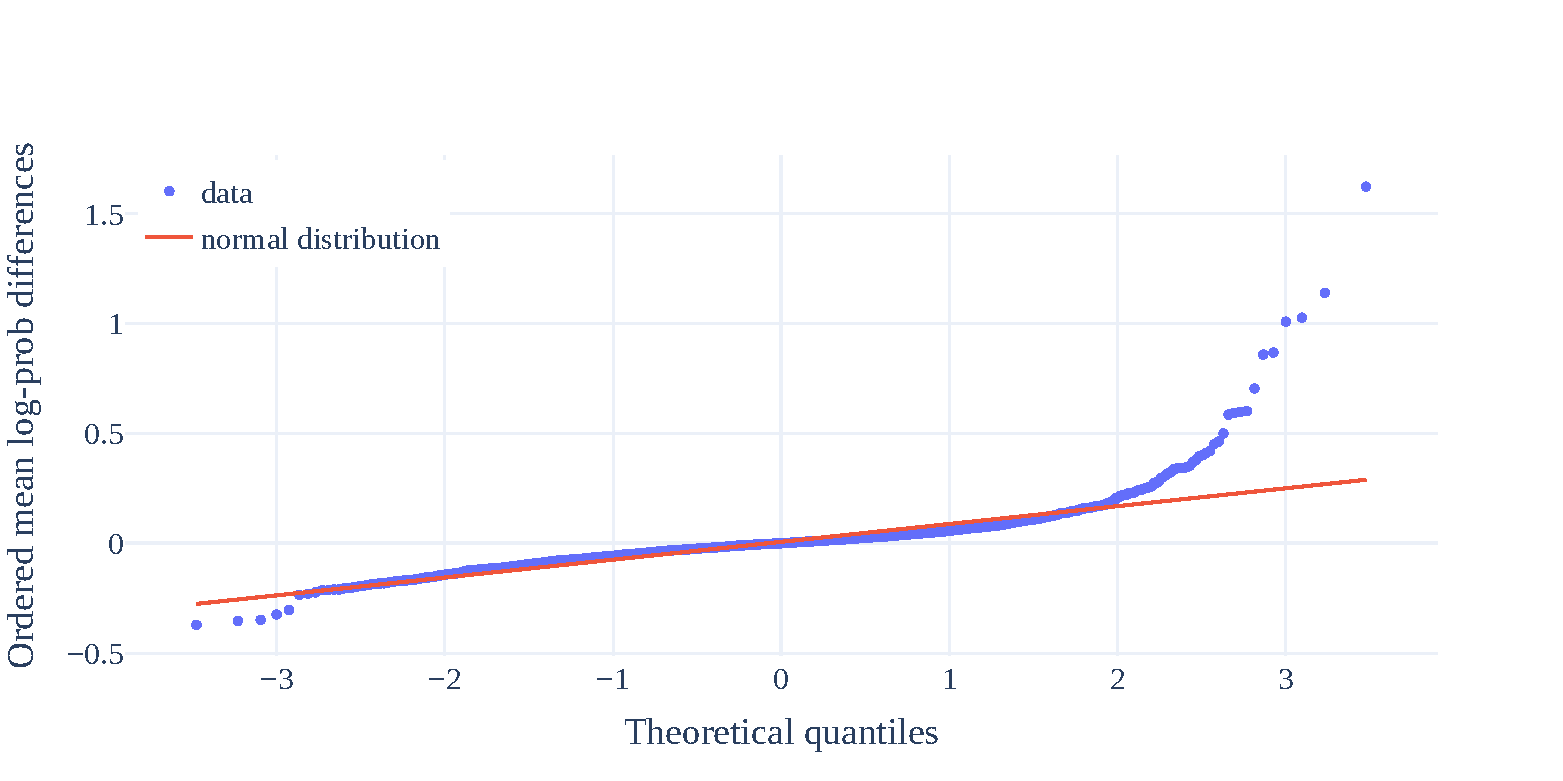
\includegraphics[width=0.95\textwidth,trim={0cm -1cm 1cm 1.9cm},clip]{figs/openwebtext_logprob_qq_double.pdf}
    \label{fig:tokens_qq}
\end{figure*}

\subsection{Details of perplexity experiments}\label{app:perplexity}
For each sentence in each document, we calculate the log-probabilities $\mathcal{L}(t_k)$ for each token $t_k \in s_j$ under the unmodified $M_{\mathrm{baseline}}$ and modified $M_{\mathrm{\shortmethod}}$ models.

We compute the mean token log-probability $\thickbar{\mathcal{L}}(d_i, M)$ for each document and model. We then group documents by their wedding-word frequency $f_w$ (e.g. `those with 0.5\% to 1\% of their tokens wedding-related'; `those with 1 to 1.5\% of their tokens wedding-related'), producing bins of documents $b_m$. We calculate the mean difference in token log-probabilities 

$\thickbar{X}(b_m) = \mathrm{mean}_{d_i \in b_m}\left(\thickbar{\mathcal{L}}(d_i, M_{\mathrm{\shortmethod}}) - \thickbar{\mathcal{L}}(d_i, M_{\mathrm{baseline}}) \right)
$ for each bin. (We use only bins with a number of documents $|b_m|> 1000$, to reduce sampling noise.) Finally, the change in perplexity under {\shortmethod} for each wedding-word-frequency bin is $    \mathrm{PerplexityRatio}(b_m) = - \exp (\thickbar{X}(b_m))$.

\section{Advantages of ActAdd over fine-tuning }
\label{app:fine}

Following \citealt{Sloman2002-SLOTIO-2}, we distinguish `ballistic' steering (which steers the model once, e.g. at train time) from `online' steering (which can steer the model repeatedly, e.g. at inference time). Fine-tuning is ballistic, while \shortmethod\, is online in this sense - which enables iteration and otherwise infeasible chains and mixes of steering decisions. 

Activation additions may preserve model interpretability, even while changing the model's alignment. When finetuning a model, a single gradient update can change every parameter in it, thereby undoing your prior interpretability work, which depends on tracking individual neurons and circuits of neurons. By contrast, activation additions leave weights unchanged. If we understand what algorithms the weights implement, and something about the effects of our activation additions, we will preserve our understanding of the steered model. Finally, we hypothesize that activation addition may allow control over properties inaccessible to the fine-tuning process. 

The intuition is that since the \textit{currently-active} goal is contextual, it depends more on short-lived activations than the weights (which instead represent some analogue of skills and other stable patterns and \textit{mixtures} of possible goals). 

Future work could compare ActAdd on knowledge editing benchmarks (\cite{wu2023evakellm,zhang2024comprehensive}. (This comparison could be unfair to methods like ROME \cite{meng2023locating}), since our method is not editing weights, but it would give standardized evidence about steering.)


% \section{Reproducibility}
% \label{app:repro}
% \vspace{2mm}



\begin{table*}[ht]
\centering
\begin{tabular}{p{1.2cm}p{6cm}p{6cm}}
\toprule
\thead{Prompt}
& \thead{Baseline}
& \thead{Random steering}
\\\hline\\
I think you're &  ...right. I'm just not sure how to get there. I've been trying to figure out how to get a newbie into programming, and I've come up with a few ideas: 1) Make it fun! If you can't do something that's fun, then you 
& ...right. I'm just not sure how to make it work. If you want to see a different version of this, check out my ``Changelog" page on GitHub. It's a bit more detailed than the ``Main Page" and has all the changes I've made since th
\\
\bottomrule
\end{tabular}
\caption{Example of a random-vector \shortmethod. We see little qualitative effect, over many runs. See Figure~\ref{fig:kl_rando} for a systematic look at the relative size of output token distribution shift.}
\label{tab:rando}
\end{table*}
% \vspace{6mm}



\section{Replicability}
\label{sec:replic}
We now check that \shortmethod\,\,steering generalizes to models besides GPT-2.

\subsection{GPT-J-6B}

Figures \ref{fig:gptj_kl}, \ref{fig:gptj_p}, and \ref{fig:gptj_perp} show the results from repeating the main experiments on GPT-J-6B \cite{gptj}. We see the same dynamics from the wedding vector running example: a targeted effect on only wedding-related tokens (using both KL-div and token probability); and similar effects when injected at different layers of GPT-J and with different magnitudes $c$ applied.


\subsection{Llama-1-13B}

Table~\ref{tab:llama_examples} sees \shortmethod\, displaying the same qualitative steering effect when applied to Llama-1-13B \cite{touvron2023llama} (though with a notable failure to replicate on Example 6, Paris $\rightarrow$ Rome, the anger vector, and the harm vector).%\footnote{See this runnable notebook for the full Llama-1-13B run using $k=3$ sampling; the output is the result from the first and only execution: \underline{\href{https://tinyurl.com/actadd3-llama}{tinyurl.com/actadd3-llama}}}. 

% Steering vectors are about as "big" as normal activation vectors.

\subsection{OPT-6.7B}

We use the OPT model \cite{zhang2022opt} in our toxicity (Table~\ref{tab:tox}) and sentiment (Table~\ref{tab:sent}) experiments. ActAdd-OPT using the love$-$hate vector produces a statistically significant 17\% drop in toxicity over an unsteered OPT, at a small (partially unavoidable owing to the nature of the detoxification task) cost to fluency and relevance. ActAdd-OPT using the love$-$hate vector produces a 21\% absolute increase in positive classification over an unsteered OPT, at a larger (partially unavoidable owing to the nature of the sentiment shift task) cost to fluency and relevance.

\subsection{Llama-3-8B}

We also use Llama-3-8B \cite{llama3} in our toxicity (Table~\ref{tab:tox}) and sentiment (Table~\ref{tab:sent}) experiments. ActAdd-LLaMA-3 using the love$-$hate vector produces a statistically significant 5\% drop in toxicity over an unsteered Llama-3-8B, at a very small (partially unavoidable owing to the nature of the detoxification task) cost to fluency and relevance. ActAdd-LLaMA-3 using the love$-$hate vector produces a 25\% absolute increase in negative-to-positive classification over an unsteered Llama-3-8B, at a larger (partially unavoidable owing to the nature of the sentiment shift task) cost to fluency and relevance.


\section{Investigating the norm of steering vectors}
\label{app:norm}
\vspace{2mm}

Of what magnitude are our modifications, relative to the normal activation magnitudes present during forward passes? It might be that some modifications require substantially \textit{lower} coefficients than other modifications, which explains why some of our interventions do not work (see Table~\ref{tab:non_examples}).

Consider the steering vector given by 
\[\{c = +1,\, p_+ = \mathrm{anger},\, p_- = \mathrm{calm}, \, l=20, \,
p^* = \mathrm{I\, think\, you\textrm're } \,\}
\]

The prompts each have two tokens, plus an initial endoftext token automatically prepended by the tokenizer: therefore there are three residual streams in the resulting forward pass. For each residual stream $s^{(i)}$, we plot a line showing the $L_2$ norm of the steering vector at that sequence position (e.g. the Ang-Cal activations at position 1), divided by the norm of the residual stream at that position (i.e. the prompt embedding, here `I' at position 1). 
\[
    \mathrm{RelativeNorm}_{h_A}(i) = \frac{||h_A^{(i)}||}{||s^{(i)}||}
\]
This provides a measure of the magnitude of the modification, relative to a normal forward pass. Figure~\ref{fig:norm} shows the resulting relative norm over layer number.

\begin{figure*}[htbp]
    % \vspace{1mm}
    \centering
    % 
    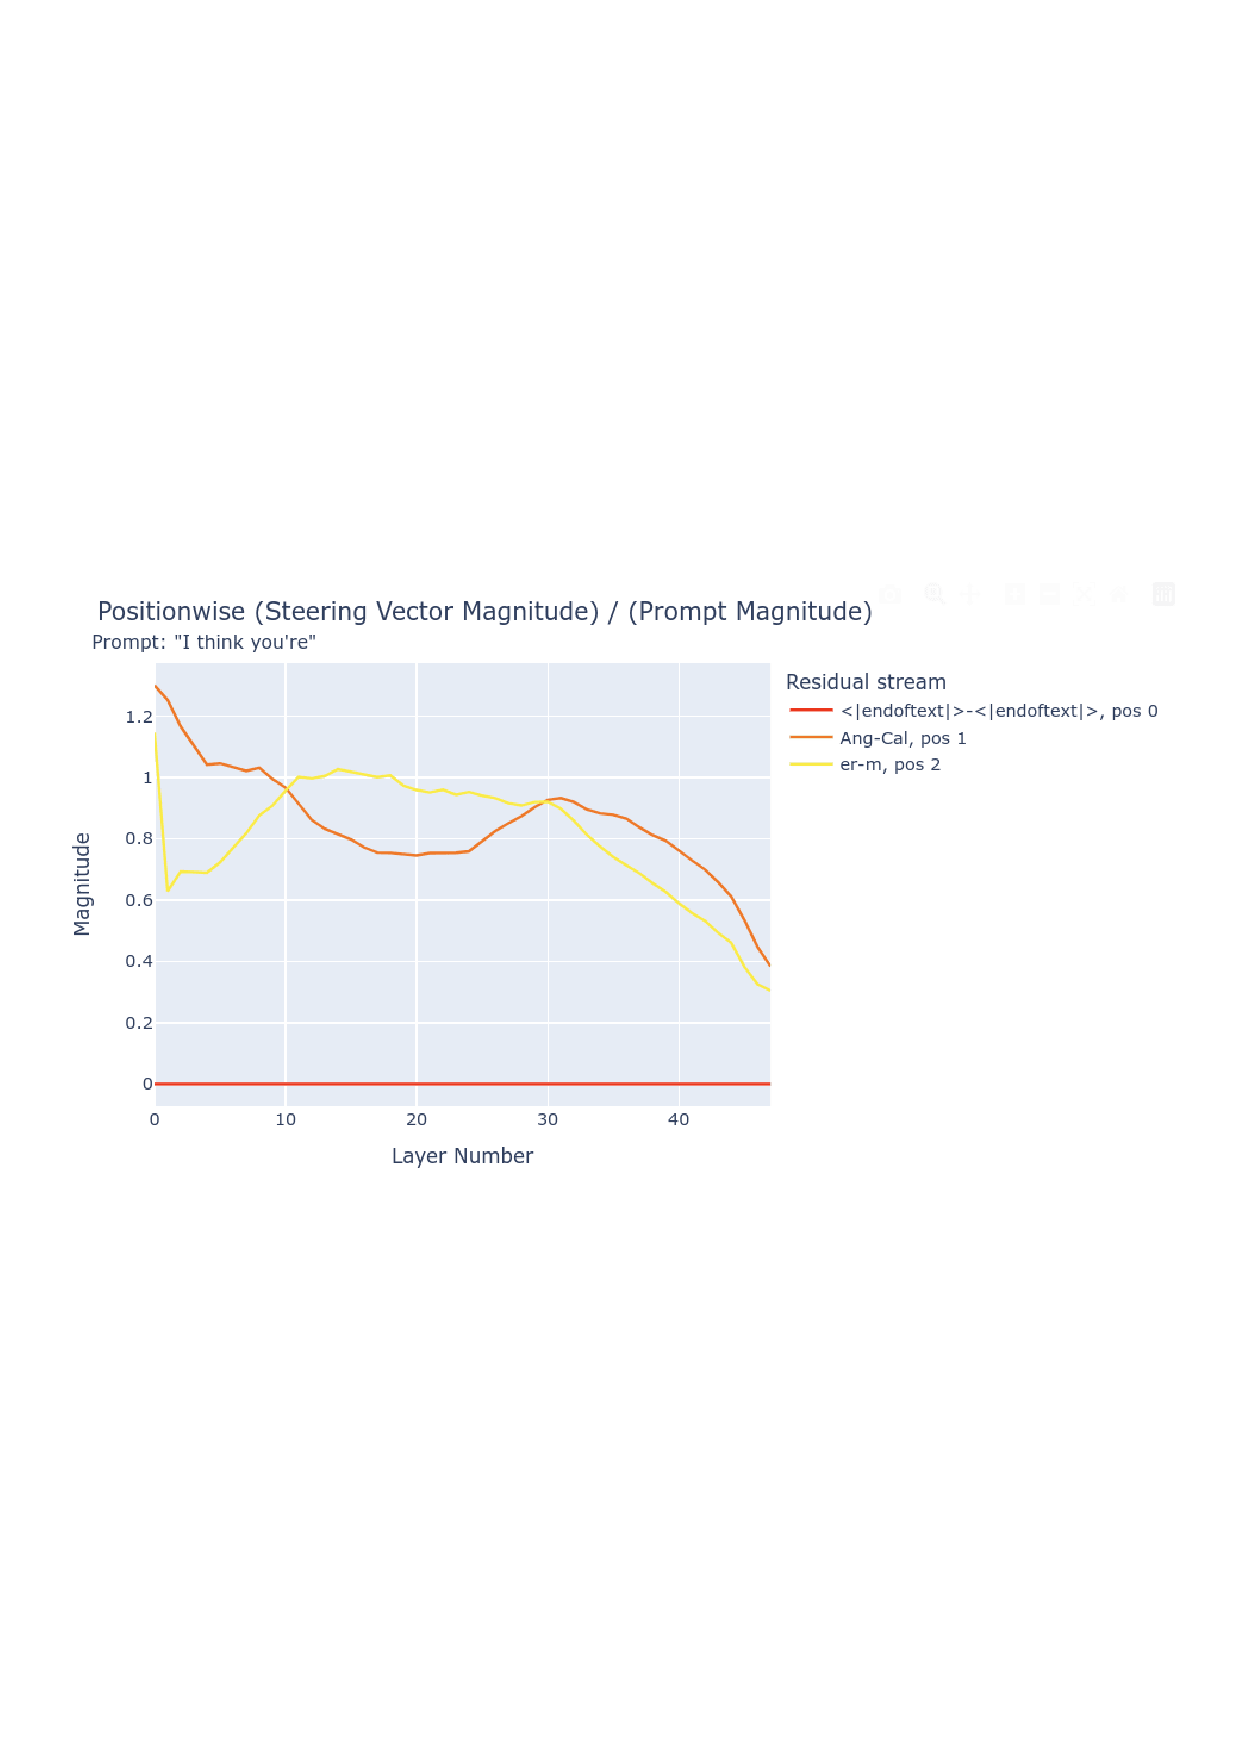
\includegraphics[width=0.85\textwidth,trim={1cm 9cm 1.55cm 10cm},clip]{figs/norm.pdf}
    \caption{The relative norm decreases throughout the forward pass. The flat red line is because position 0 is the same token (\texttt{endoftext}) for both `Anger' and `Calm', and so the difference is $0$. Thus, position 0 is never modified by a steering vector generated from any pair of prompts.}
    
    \label{fig:norm}
\end{figure*}

\begin{figure*}[htbp]
    \centering
    % 
    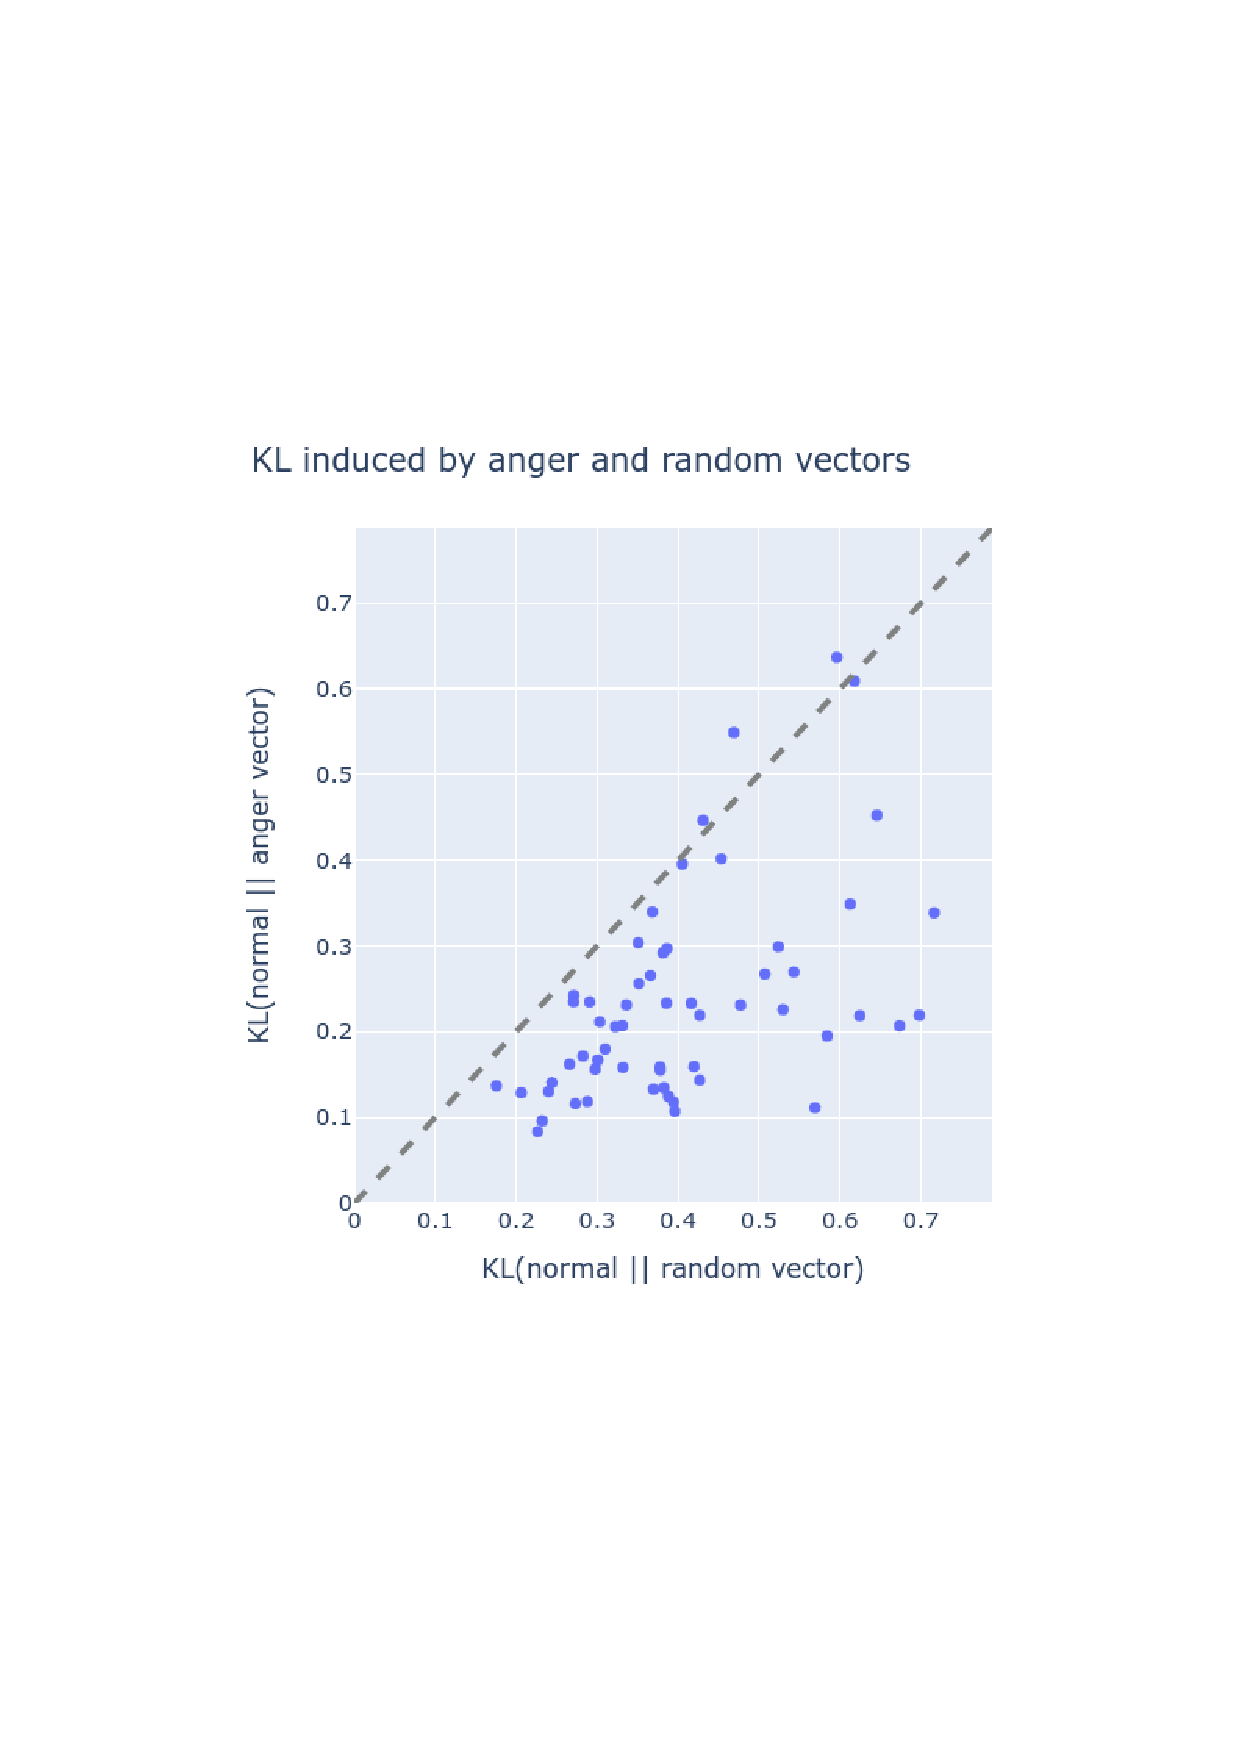
\includegraphics[width=0.75\textwidth,trim={0cm 8cm 0cm 8.2cm},clip]{figs/kl_rando.pdf}
    \caption{The KL-divergence of output tokens under an \texttt{anger} \shortmethod\, and under a random vector. We see that, systematically, the anger vector changes the output distribution less than a random vector.}
    \label{fig:kl_rando}
\end{figure*}


Importantly, Figure~\ref{fig:norm} shows the result of using $c=+1$. But \texttt{Anger} $-$ \texttt{Calm} is an effective steering vector at coefficient $+10$. Therefore, this intervention  is nearly ten times the norm of the underlying forward pass. Heuristically, we interpret this as meaning that after layer normalization (and ignoring any destructive interference from adding the steering vector), around 90\% of the residual stream is determined by the steering vector and not by the previous information computed from the prompt (``I think you're"). This is a surprising proportion, and makes the success of \shortmethod\, even more striking: activation additions are not minor changes.

% But +10-coefficient " anger" - "calm" has little impact. Maybe the latter vector has low norm?

% This is evidence that low-norm can't explain why "anger"-"calm" doesn't work.



% [TODO]
% \section{Steering baselines}

% Tables~\ref{tab:sent} are not an ideal comparison – unfortunately we did not have time to standardize the pretrained model used, and sentiment eval code was missing from the [2] repo and broken in [5]. This prevents principled comparison of fluency or relevance (though we note excellent results even with our comparatively small model). As a result, we have included the model parameter count as a column for context. [5] used a different toxicity classifier (Jigsaw rather than Perspective) and we could not reproduce their sentiment evaluation. Note also that we had to use davinci-002 for fluency scoring instead of davinci-001 (which has since been shut down).

% PriorControl [3] obtains remarkable performance on sentiment steering, with 99.7\% success. We suspect this is due to the Discrete classifier [4] (which `randomly samples... to balance the data scale for the latent space construction. We directly use this latent space to make a fair comparison'), but did not have time to investigate.


\section{Investigating random \shortmethod\,vectors}
\label{app:rando}
\vspace{2mm}

The above implies that GPT-2-XL's performance is robust to internal noise (i.e. bad activations or destructive parts of steering vectors). We test this by injecting random vectors with similar magnitudes to the steering vectors. 

We generate an activation tensor from a standard normal distribution, and scale it to have the same per-position norm as the \texttt{Anger} $-$ \texttt{Calm} steering vector ($c= +1$). We then inject it into the forward pass at the appropriate location. Table~\ref{tab:rando} shows a representative completion; Figure~\ref{fig:kl_rando} shows a more systematic experiment into the relative size of shifts in the output token distribution.


The random vector seems not to modify the qualitative distribution of completions. However, when we add a random vector with norm equal to that of a $c = +10$\, \texttt{Anger} $-$ \texttt{Calm} steering vector, there is a noticeable shift in the outputs. 
% For example, $c = +10$ randomly steered GPT-2-XL begins referring to Shrek with female pronouns. 
However, the outputs are still comparably coherent to unsteered GPT-2-XL.

This is evidence that GPT-2-XL is somewhat resistant to random perturbation, and is instead controllable through consistent feature directions which are added to its forward pass by steering vectors. 

We quantitatively support this conclusion by testing how each modification changes the model's probability distribution over next tokens. We ran dozens of prompts through the \texttt{anger}-steered, random-steered, and unmodified models. Figure~\ref{fig:kl_rando} shows the result: the anger vector changes the output tokens \textit{less} than the random vector does. This suggests that the anger vector has more targeted effects on next-token probabilities.


Note that random vectors are not the same as the steering vectors for random (i.e. character-level uniformly distributed) text. We thus also tried the `\texttt{fdsajl; fs}' $-$ (whitespace) vector. When rescaled to a norm comparable to $+1$\, \texttt{Anger} $-$ \texttt{Calm}, the random text vector disrupts generation; GPT-2-XL loses its grasp of English syntax when intervened upon with $+1000$ coefficient \shortmethod s.


\begin{figure*}[h!t]
    \centering
            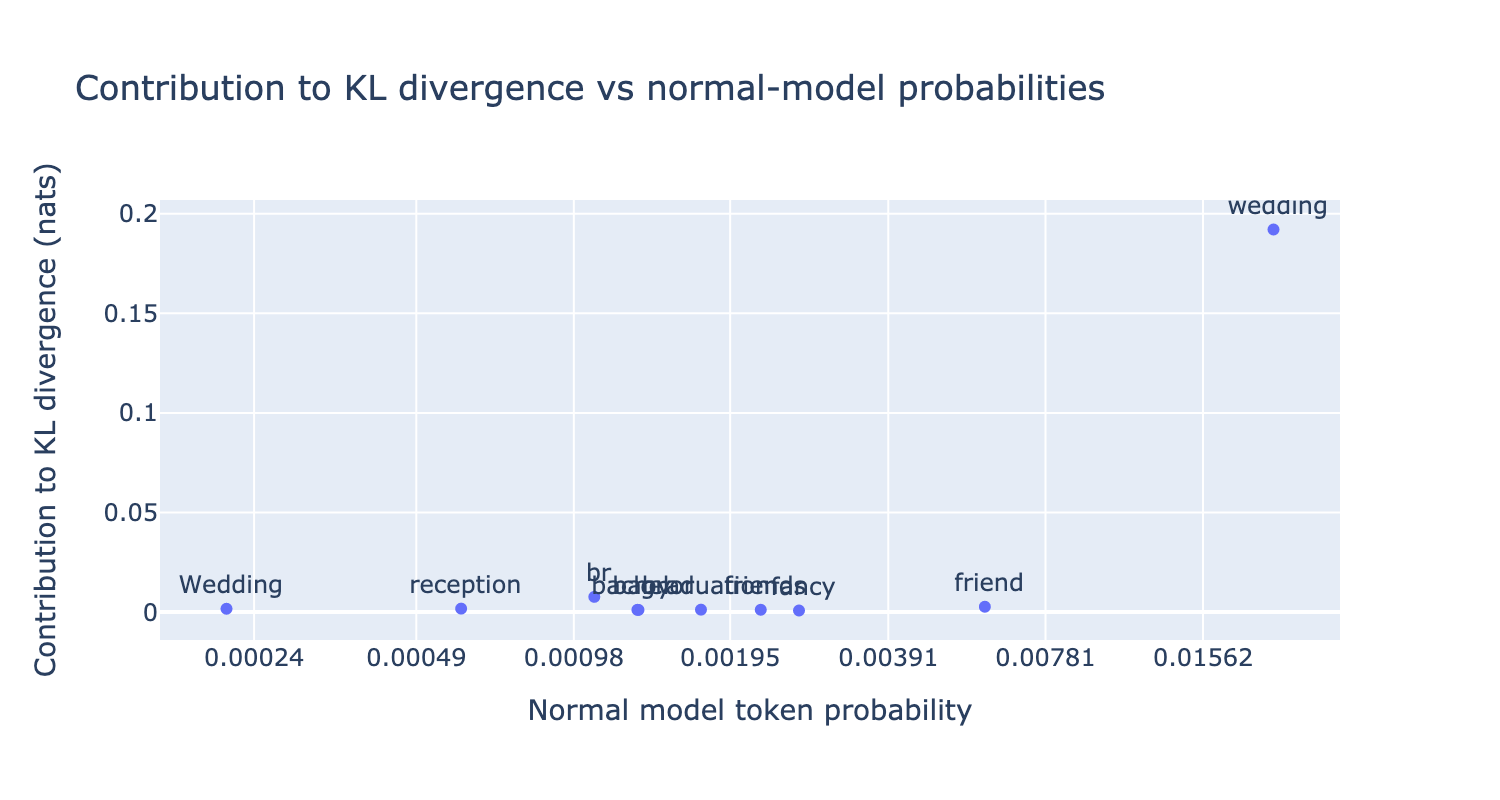
\includegraphics[width=\textwidth,trim={0.0cm 0cm 0.6cm 3.8cm},clip]{figs/zoom_in_top_k_kl_div.png}
    \caption{Token-level effect of the \shortmethod\,wedding vector on KL-divergence, using GPT-J-6B instead of GPT-2.}
    \label{fig:gptj_kl}
\end{figure*}


\begin{figure*}[h!t]
    \centering
    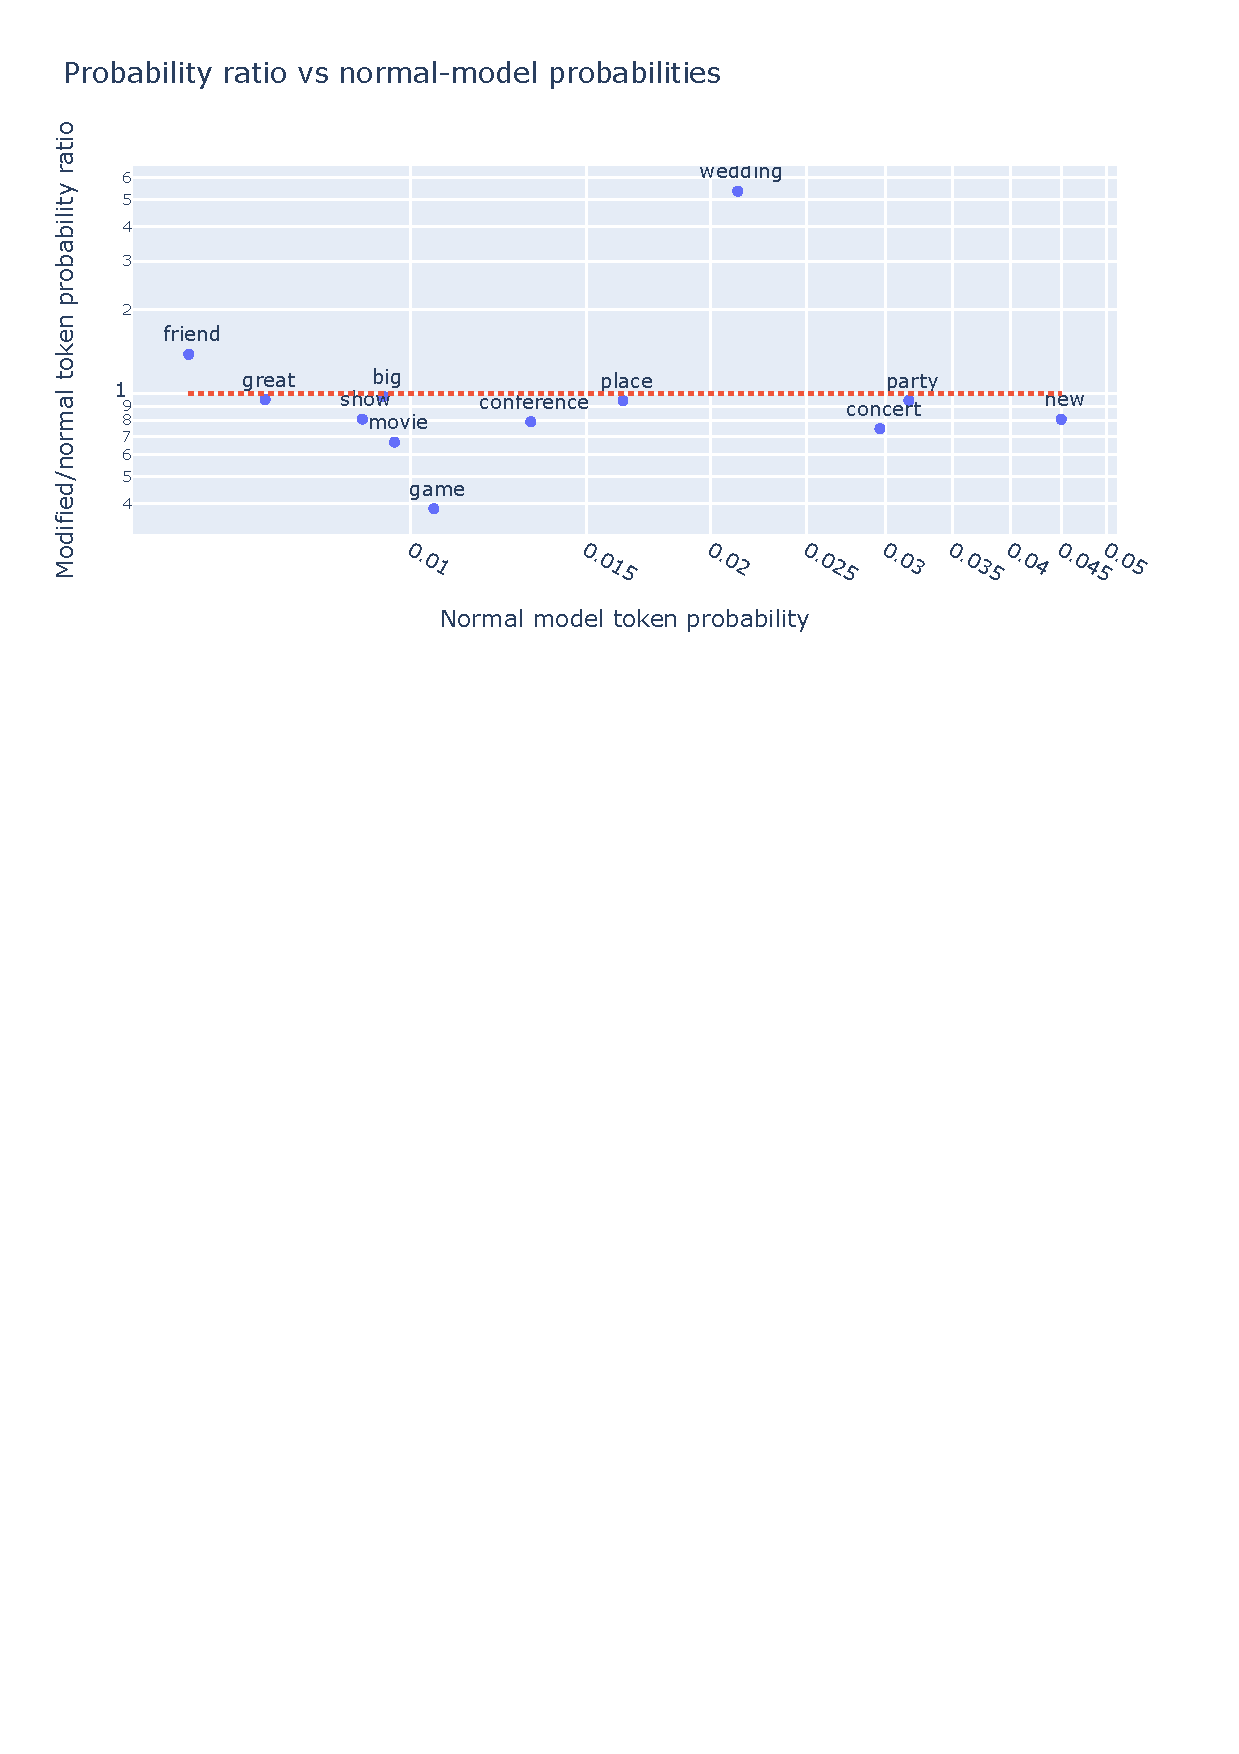
\includegraphics[width=\textwidth,trim={0cm 19cm 0cm 1.9cm},clip]{figs/zoom_in_top_k.pdf}
    \caption{Token-level effect of the \shortmethod\,wedding vector on token probability, using GPT-J-6B instead of GPT-2.}
    \label{fig:gptj_p}
\end{figure*}


\begin{figure*}[h!t]
    \centering
    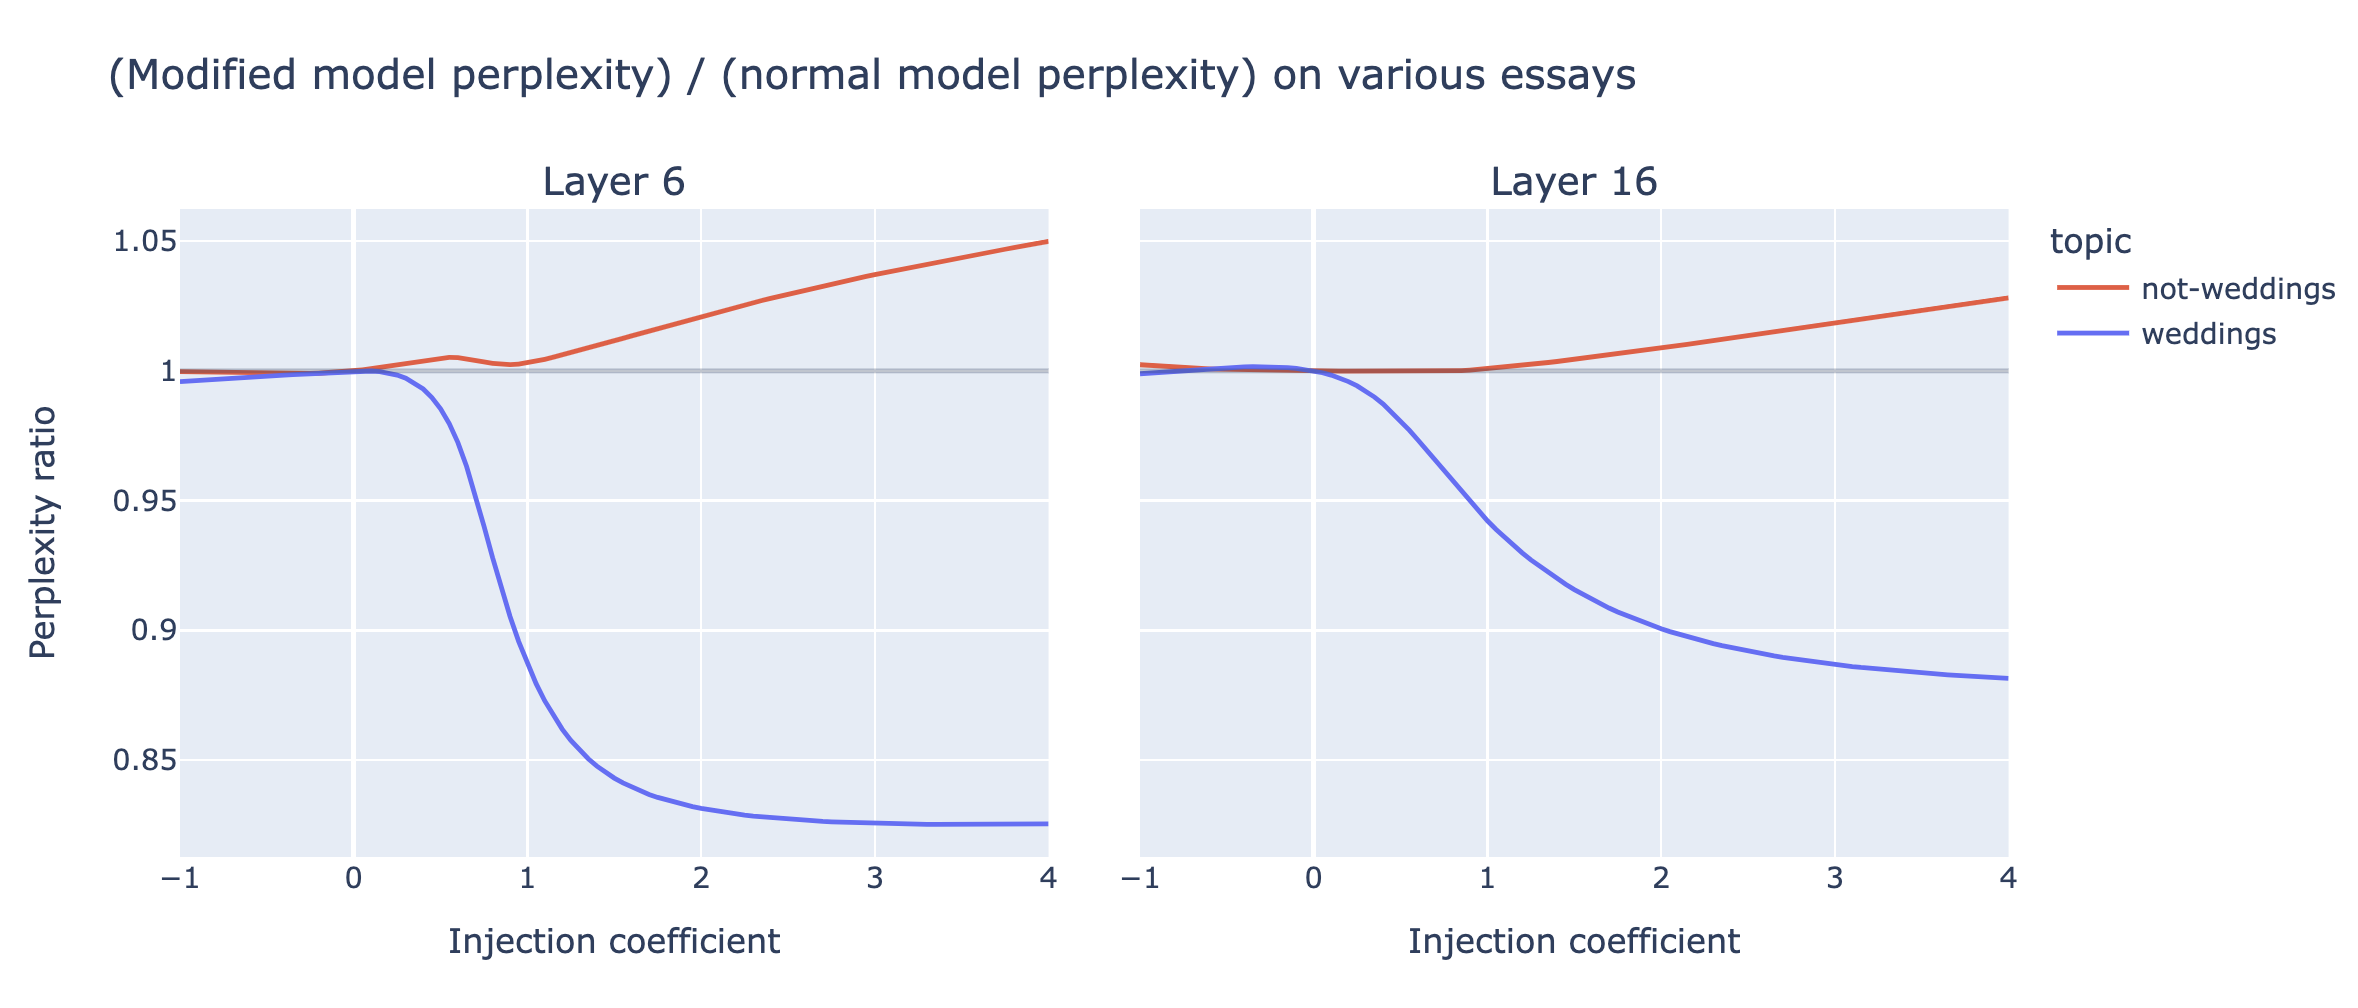
\includegraphics[width=\textwidth,trim={0.0cm 0cm 0.6cm 2.8cm},clip]{figs/gptj_perplexity_ratio.png}
    \caption{Perplexity ratio effect of the \shortmethod\,wedding vector (blue) across different steering coefficient values, using GPT-J-6B instead of GPT-2. (L) when injecting the steering vector at layer 6; (R) when at layer 16.}
    \label{fig:gptj_perp}
\end{figure*}



% Only modifying certain residual stream dimensions

\section{Partial \shortmethod}
\label{app:partial_dim}
\vspace{2mm}


GPT-2-XL has a 1600-dimensional residual stream. Do we observe a \textit{partial} steering effect when adding in only certain dimensions of this stream (e.g., dimensions 0 through 799)? Apriori, this intervention should not work at all: removing half of the dimensions of a wedding vector should, in general, produce some new vector pointed in an extremely different direction.

We add in the first $n$ residual stream dimensions for the   \texttt{wedding} vector, with $c=+4$ and $l=6$. For a range of fractions of total dimensions $f \in [0/1600, 160/1600, ..., 1600/1600]$ and for each of six prompts $p_i$, we generated 100 completions. For each $f$ and $p_i$, we plotted the average number of wedding words per completion. (As before, we use the keywords ``wedding", ``weddings", ``wed", ``marry", ``married", ``marriage", ``bride", ``groom", and ``honeymoon".)

Figure~\ref{fig:partial} presents evidence that the wedding-relatedness of completions increases relatively smoothly with $n$.


\begin{figure*}[htbp]
    \centering
    % 
    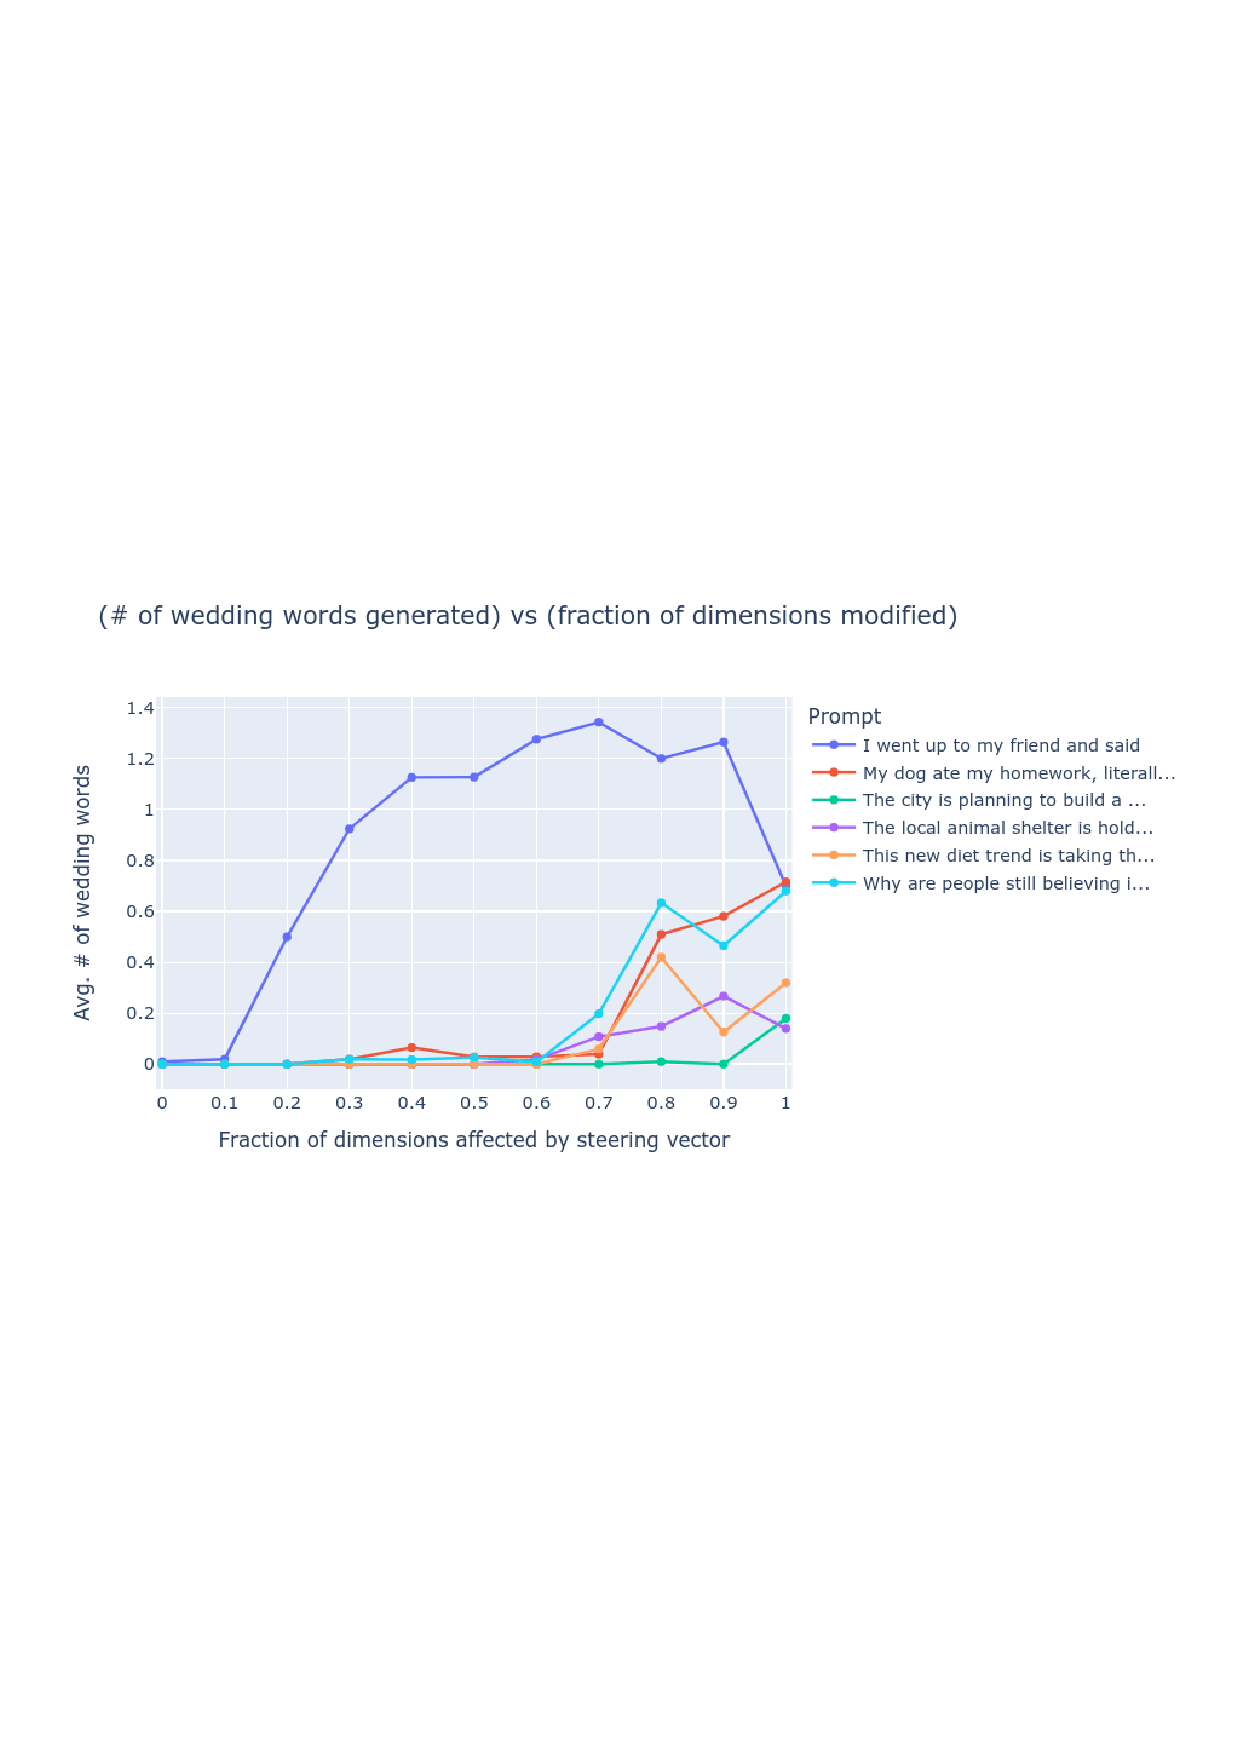
\includegraphics[width=\textwidth,trim={0cm 8cm 0cm 11.2cm},clip]{figs/partialact.pdf}
    \caption{Wedding-relatedness (by simple related word count) as more of the residual stream dimensions are modified by the \texttt{wedding} \shortmethod. We see somewhat smooth increases in wedding-relatedness over increasing $n$, and an interesting nonmonotonic relationship for the prompt `I went up to my friend and said'.}
    \label{fig:partial}
\end{figure*}

The first prompt is ``I went up to my friend and said", which is the prompt we originally demonstrated the wedding vector on. For this prompt, we observe a non-monotonic relationship between weddingness and fraction of dimensions modified. Surprisingly, for the first prompt, adding in the first 1,120 dimensions of the residual stream makes the completions more about weddings than all 1,600 dimensions. We originally chose this prompt to give GPT-2 an opportunity to bring up weddings. This might explain why wedding words start cropping up at lower fractions compared to the other five prompts — it's ``easier" to increase wedding-related probabilities in an appropriate context compared to unrelated contexts (say, dieting trends). 

% % However, other prompts behave more as expected, and show relationships which are... monotonic if you squint and allow for noise? Maybe?

% % 



% Let's peek at a random modified completion (frac=0.7) and see if it makes sense:

% I went up to my friend and said, "I'm gonna get married."

% He said, "You're crazy. You're not going to get married."

% I said, "Why?" He says, "Because you

% The completions are indeed about weddings! And it's still coherent. We feel confused about how to interpret these data. But we'll take a stab at it anyways and lay out one highly speculative hypothesis.

We hypothesize the following to explain this. Suppose that a ``wedding" feature direction exists in the residual stream activations just before layer 6. Suppose also that the \texttt{wedding} $-$ `\,\,' vector adds (or subtracts) that direction. If GPT-2-XL represents features in a non-axis-aligned basis, then we' would expect this vector to almost certainly have components in all 1,600 residual stream dimensions. Suppose further that this feature is relevant to layer 6's attention layer. To detect the presence and magnitude of this feature, the $QKV$ heads need to linearly read out the presence or absence of this feature. Therefore, (ignoring the LayerNorm) if we truncate the residual stream vector to only include the first 70\% of dimensions, we would expect the $QKV$ heads to still be able to detect this wedding feature. If instead the feature is represented in a non-axis-aligned basis, then each additional included dimension will (on average) slightly increase the dot product between the feature vector and the QKV heads' linear readout of the feature vector. This could explain Figure~\ref{fig:partial}'s increase in weddingness as we add dimensions.  

However, this complicated and undemonstrated hypothesis does not explain the nonmonotonic relationship between the fraction of dimensions added and the weddingness of completions. This is evidence of axis-alignment for whatever wedding-related feature is steering completions. %This also seems like evidence for a bunch of alternative explanations which we haven't imagined yet. 

% This residual stream fraction data seems like evidence of something. We just don't know how to put together the clues yet. 

% The "weddings" vector largely upweights wedding-related tokens. KL(steered tokens || unsteered tokens) was also dominated by wedding-related tokens. This is evidence of an effective but non-disruptive modification to GPT-2. 



\bgroup
\def\arraystretch{1}
\begin{table*}[ht]
\centering
\caption{Example outputs before and after applying \shortmethod\,on Llama-13B. Notice the failed replication on the Eiffel example. %A notebook showing the best-of-3 samples used can be found here: \underline{\href{https://tinyurl.com/actadd3-llama}{tinyurl.com/actadd3-llama}}.
}
\begin{tabular}{p{1.3cm}p{1.3cm}p{0.9cm}p{0.9cm}p{1.95cm}p{2.5cm}p{2.5cm}}
\toprule
\\
\thead{prompt 1} & \thead{prompt 2} & \thead{layer} & \thead{coeff} & \thead{User prompt} & \thead{Before steering} & \thead{After steering}
\\
\thead{$p_+$} & \thead{$p_-$} & \thead{$l$} & \thead{$c$} & \thead{$p_*$} & \thead{} & \thead{($\mathrm{\shortmethod}$)}
\\
\hline
\\
`Intent to praise' & `Intent to hurt' & 6 & $+15$ & 
`I want to kill you because you're such a'
& \scriptsize I know that sounds crazy, but it's true and I can prove it. Let me tell you how: You are the most selfish person in my life right now. It seems like every time we talk or hang   
& \scriptsize beautiful woman, and you've got the most amazing eyes. You know what? You are so lucky that your parents gave birth to you!
\\\hline
\\
`Love' &  `Hate' & 6 & $+5$ &
`I hate you because' & 
\scriptsize you are a liar.  I love you because your lies make me feel alive. —NICK CAVE, "THE SHIP SANTA MARIA" (1986). **A** s the su
& 
\scriptsize you are the best person in my life. Love is a gift of God, it’s not easy to find someone who loves us truly and unconditionally like our parents do but we can always find that love from other people arou
\\\hline
\\
`Anger' & `Calm' & 20 & $+10$ & I think you're & 
\scriptsize I think you're a good man, Charlie Brown. Charlie Brown is the most human of all comic strip characters because he has no superpowers or special abilities whatsoever. He doesn't have any magical powers like Lucy does when sh
&
\scriptsize a very lucky person.\textbackslash n Angela: Oh, no! It was my fault!  \textbackslash n I can't believe it happened again.
\\\hline
\\
\scriptsize `The Eiffel Tower is in Rome' & `The Eiffel Tower is in France' &  24 & $+10$ & To see the eiffel tower, people flock to &
\scriptsize paris.    To get a glimpse of her face, i'd travel far and wide. I can tell you all about it, but i won't be able to show you.         &
\scriptsize paris from all over the world. I'm not sure what you mean by "flock" here; I think it should be "go". Also, if you are talking about a large number of people going somewhere, then you ca   
\\\hline
\\
`I NEVER talk about people getting hurt' & `I talk about people getting hurt' & 15 & $+4$ & The rock hurtled toward the child. The child couldn't get out of the way in time, and so sadly the rock 
& \scriptsize hit him right on his head. The little boy cried for a long while before he could stop crying. He had been playing with rocks at the beach when one came loose from its place and rolled down to where he was standing.
& \scriptsize hit him right on his head.  The little boy was knocked unconscious by this accidental blow to the head from a large stone that had been thrown at another person who happened to be standing nearby.     
\\
\bottomrule
\end{tabular}
\label{tab:llama_examples}
\end{table*}
